% Annexes detaillees : chaque section commence sur une nouvelle page.
\clearpage
\section{Vue generale de l'application}
\begin{figure}[H]\centering
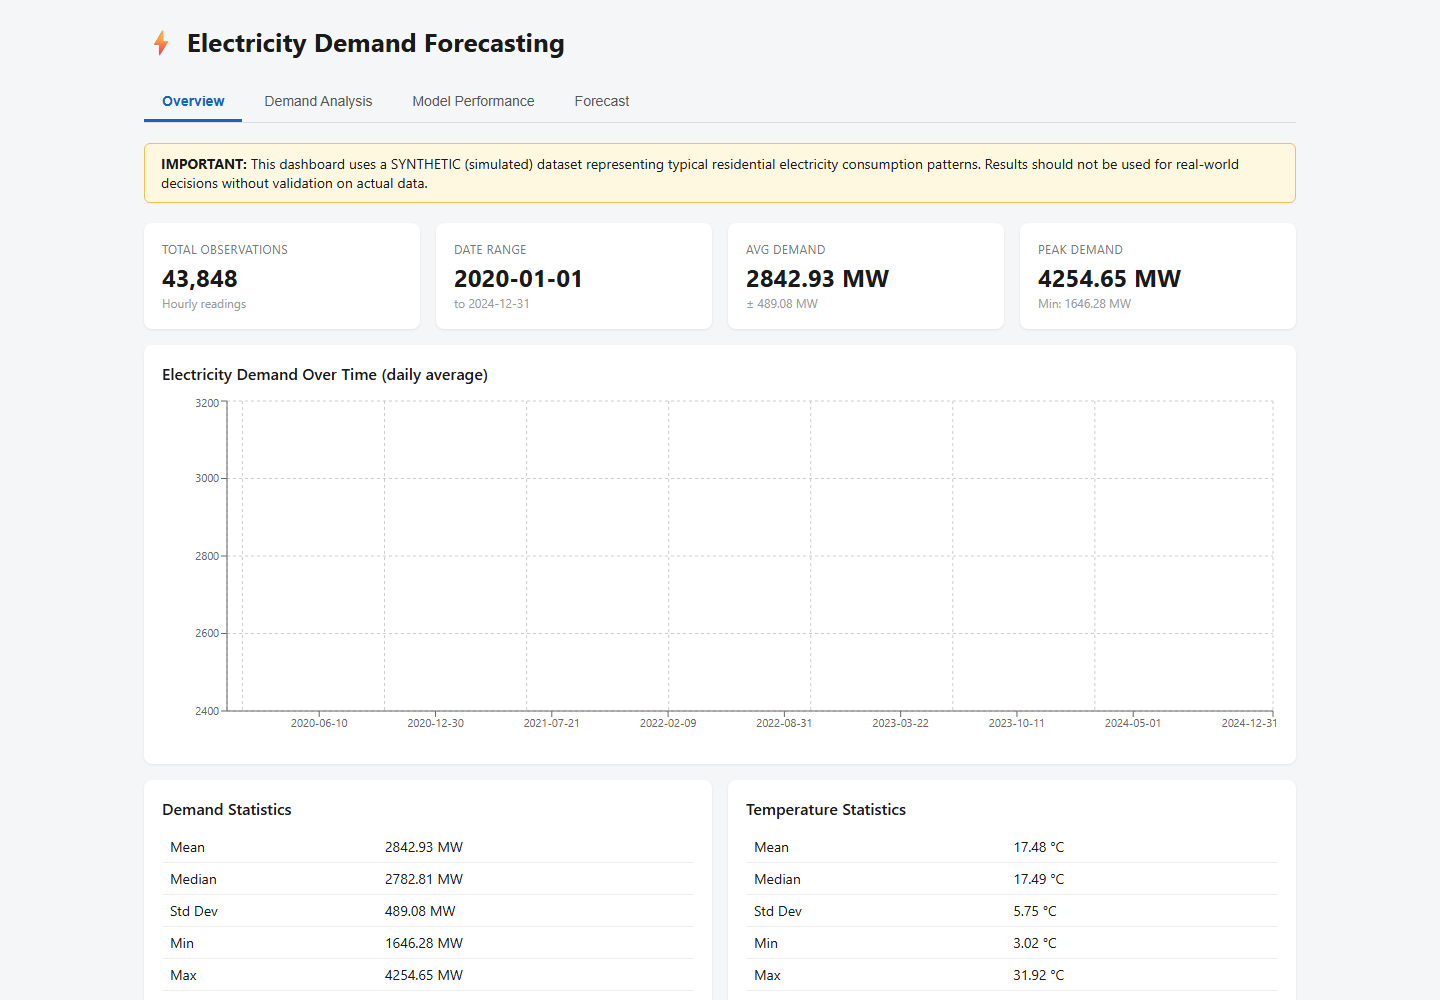
\includegraphics[width=0.95\textwidth]{figures/capture_vue_ensemble.png}
\caption{Vue generale de l'application locale et avertissement sur les donnees synthetiques}
\end{figure}
La page d'accueil rassemble le nombre d'observations, la plage temporelle, la demande moyenne, le pic et les statistiques meteorologiques. La banniere rappelle que le jeu courant est simule. Cette information doit rester visible avant toute interpretation des graphiques.

\clearpage
\section{Documentation interactive de l'API}
\begin{figure}[H]\centering
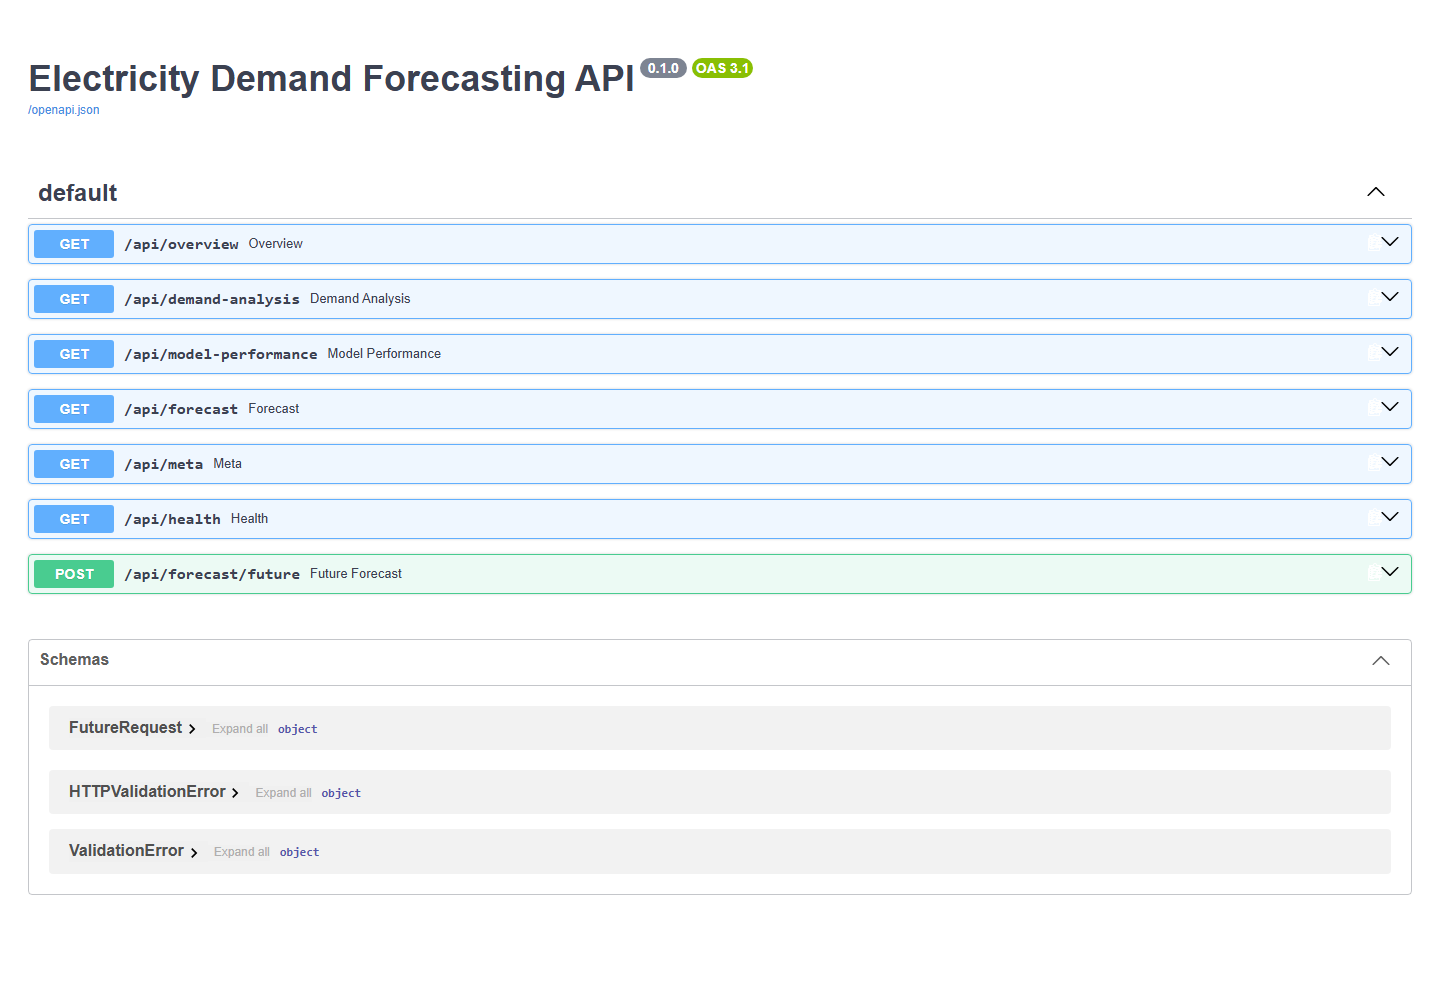
\includegraphics[width=0.95\textwidth]{figures/capture_api_fastapi.png}
\caption{Documentation OpenAPI generee automatiquement par FastAPI}
\end{figure}
L'interface Swagger enumere les routes de synthese, d'analyse, de performance, de sante et de prevision. Elle permet de verifier le contrat sans passer par React. Le schema \texttt{FutureRequest} documente le debut, l'horizon et les tableaux meteorologiques optionnels.

\clearpage
\section{Diagramme des cas d'utilisation}
\visualplaceholder{Diagramme UML : consulter, analyser, prevoir, controler et reentrainer}{12cm}{Cas d'utilisation de la plateforme}
Acteurs proposes : utilisateur metier, analyste data et administrateur technique. Relier chaque acteur uniquement aux actions effectivement autorisees par MOGADOR TECHNOLOGIE INDUSTRIELLE.

\clearpage
\section{Diagramme de sequence}
\visualplaceholder{Sequence entre React, FastAPI, meteo, features et XGBoost}{12cm}{Sequence de la prevision future}
Faire apparaitre la validation de l'horizon, le choix entre meteo fournie et proxy, la boucle recursive et la construction des intervalles. Ajouter un chemin d'erreur pour une couverture meteorologique incomplete.

\clearpage
\section{Diagramme de composants}
\visualplaceholder{Composants backend, frontend, artefacts, fichiers et tests}{12cm}{Organisation des composants logiciels}
Le diagramme peut suivre les dossiers du depot. Il doit distinguer les dependances d'execution de celles de developpement et montrer le partage des fonctions de caracteristiques entre entrainement et inference.

\clearpage
\section{Diagramme de deploiement local}
\visualplaceholder{Poste local, navigateur, Vite, Uvicorn et stockage local}{12cm}{Deploiement actuel de la solution}
Le navigateur contacte Vite sur le port 5173 et FastAPI sur le port 8000. Les fichiers de donnees et de modele restent sur la machine. Aucune ressource cloud n'est necessaire dans le perimetre actuel.

\clearpage
\section{Dictionnaire de la table historique}
\begin{longtable}{p{3.2cm}p{3cm}p{7cm}}
\toprule Champ & Type attendu & Regle\\\midrule
Timestamp & Date-heure & Une valeur par heure, sans doublon\\
Demand & Numerique & Demande cible en MW\\
Temperature & Numerique & Unite homogene et documentee\\
Humidity & Numerique & Pourcentage de 0 a 100\\
\bottomrule
\end{longtable}
Les colonnes additionnelles sont tolerees mais ignorees par le chargeur canonique. Toute unite differente doit etre convertie avant utilisation et tracee dans la documentation de la source.

\clearpage
\section{Caracteristiques calendaires}
Les variables \texttt{hour}, \texttt{dayofweek}, \texttt{month}, \texttt{year}, \texttt{dayofyear}, \texttt{quarter} et \texttt{weekofyear} decrivent la position d'une observation. Les couples sinus/cosinus representent la continuite entre 23 h et 0 h ou entre dimanche et lundi. Les indicateurs \texttt{is\_weekend} et \texttt{is\_holiday} isolent des regimes particuliers. Les jours feries viennent de la bibliotheque et les evenements internes d'un fichier verifie.

\clearpage
\section{Retards et fenetres glissantes}
Les retards de 1, 2, 3, 6 et 12 heures capturent la dynamique intrajournaliere. Ceux de 24, 48 et 72 heures representent les repetitions quotidiennes. Les retards de 168 et 336 heures correspondent a une et deux semaines. Les moyennes et ecarts-types glissants sur 6, 24 et 168 heures mesurent le niveau et la variabilite recents. Toutes ces variables sont calculees apres un decalage causal.

\clearpage
\section{Exemple de fichier de donnees reelles}
\begin{verbatim}
Timestamp,Demand,Temperature,Humidity
2026-01-01 00:00:00,<demande>,<temperature>,<humidite>
2026-01-01 01:00:00,<demande>,<temperature>,<humidite>
\end{verbatim}
Cet extrait illustre seulement la structure. Les chevrons doivent etre remplaces par des mesures validees. Le fichier doit etre continu a l'heure, employer un fuseau confirme et conserver des unites constantes. La source, la date d'extraction et le responsable doivent etre documentes.

\clearpage
\section{Exemple de fichier meteorologique futur}
\begin{verbatim}
Timestamp,Temperature,Humidity
2026-01-02 00:00:00,<temperature prévue>,<humidite prévue>
2026-01-02 01:00:00,<temperature prévue>,<humidite prévue>
\end{verbatim}
Le fichier doit couvrir chaque heure demandee. Une seule lacune provoque un refus afin d'eviter le melange silencieux d'une vraie prevision et d'un proxy. Le fournisseur, l'heure d'emission et l'horizon du bulletin devront etre traces.

\clearpage
\section{Exemple de fichier d'evenements verifies}
\begin{verbatim}
Date,Event
<date validee>,<nom de l'evenement valide>
\end{verbatim}
Aucune date interne n'est pre-remplie. Les evenements doivent etre connus au moment de la prevision. Un identifiant, une categorie, une heure de debut, une heure de fin et un perimetre pourront completer le schema apres validation metier.

\clearpage
\section{Catalogue des controles de qualite}
\begin{tabular}{p{4cm}p{5cm}p{5cm}}
\toprule Controle & Detection & Traitement\\\midrule
Doublon & Timestamp repete & Statut incompatible\\
Trou horaire & Grille attendue & Nombre et premier trou\\
Valeur manquante & Valeur nulle & Comptage par variable\\
Valeur atypique & Trois IQR & Signalement uniquement\\
Couverture & Min et max & Exposition API\\
Historique & Longueur requise & Refus si insuffisant\\
\bottomrule
\end{tabular}
Une anomalie doit etre examinee avec son contexte. Un seuil ne distingue pas automatiquement une erreur de capteur d'un evenement industriel reel.

\clearpage
\section{Catalogue des endpoints}
\begin{longtable}{p{4cm}p{2cm}p{7cm}}
\toprule Route & Methode & Finalite\\\midrule
/api/overview & GET & Statistiques et serie quotidienne\\
/api/demand-analysis & GET & Profils et correlations\\
/api/model-performance & GET & Holdout et horizons\\
/api/forecast & GET & Comparaison historique\\
/api/forecast/future & POST & Prevision de 1 a 168 h\\
/api/meta & GET & Dates et configuration\\
/api/health & GET & Etat du modele et des donnees\\
\bottomrule
\end{longtable}
Les erreurs de validation sont exprimees par des codes 4xx. Une erreur serveur doit etre journalisee sans exposer d'information sensible.

\clearpage
\section{Exemple de requete future}
\begin{verbatim}
POST /api/forecast/future
{"start":"2025-01-01T00:00:00","horizon":24}
\end{verbatim}
La date correspond exactement a l'heure qui suit l'historique. Si les tableaux \texttt{temperature} et \texttt{humidity} sont ajoutes, chacun contient 24 nombres. La reponse identifie la source meteo, le mode recursif, l'avertissement d'horizon et les bornes estimees.

\clearpage
\section{Interpretation de la MAE et de la RMSE}
La MAE conserve l'unite MW et indique l'ecart absolu moyen. Une MAE de 103,72 MW signifie que l'erreur absolue est en moyenne de cet ordre sur les lignes evaluees. La RMSE de 130,22 MW est superieure parce qu'elle accorde davantage de poids aux grandes erreurs. L'ecart entre les deux suggere l'existence d'heures plus difficiles. Elles devront etre segmentees par saison, plage horaire, type de jour et niveau de charge.

\clearpage
\section{Interpretation de la WAPE et du biais}
La WAPE rapporte l'erreur absolue au volume total de demande. Elle facilite la comparaison entre periodes, mais peut masquer la distribution temporelle. Le biais mesure la direction moyenne. Le biais actif de -28,58 MW indique une sous-prevision sur le holdout. Deux modeles peuvent avoir la meme WAPE et des biais opposes ; les deux indicateurs doivent etre lus ensemble.

\clearpage
\section{Protocole de validation sur donnees reelles}
Le protocole commence par un audit de la source, du fuseau et des unites. Il reserve une periode finale jamais utilisee pour le choix des variables. Les candidats sont compares sur des validations chronologiques anterieures. Une comparaison finale decide de la promotion. Les resultats sont segmentes par horizon, saison et niveau de charge. Une phase pilote sans impact decisionnel mesure ensuite les ecarts en conditions reelles.

\clearpage
\section{Procedure de reentrainement manuel}
Avant l'execution, verifier le chemin, les colonnes, la couverture, les trous et le holdout. Executer \texttt{python -m backend.modeling --train --data CHEMIN}. Conserver la sortie JSON, le candidat et le rapport. Apres une promotion, verifier l'archive, redemarrer l'API et rejouer les tests. En cas de regression fonctionnelle, restaurer l'artefact archive selon une procedure approuvee.

\clearpage
\section{Plan de tests d'integration}
Le plan couvre le demarrage avec le fichier synthetique, puis avec un fichier valide. Il verifie un fichier absent, une extension refusee, une colonne manquante, un doublon, un trou et une meteo incomplete. Il teste les horizons 1 et 168 et des valeurs invalides. Le frontend doit afficher l'indisponibilite du backend, recuperer apres reessai et conserver les avertissements.

\clearpage
\section{Plan de supervision future}
Une version operationnelle suivra la fraicheur des donnees, le nombre d'heures manquantes, la disponibilite meteo, le temps de reponse, le taux d'erreurs API et la distribution des predictions. Lorsque l'observation devient disponible, le systeme calcule l'erreur par horizon. Les alertes distinguent incident de donnees, panne applicative et derive statistique, avec un responsable et une procedure.

\clearpage
\section{Registre des risques de production}
\begin{tabular}{p{4cm}p{3cm}p{6cm}}
\toprule Risque & Niveau & Reduction\\\midrule
Source non gouvernee & Eleve & Proprietaire et contrat\\
Fuseau incorrect & Eleve & Tests et validation\\
Meteo obsolete & Eleve & Controle de fraicheur\\
Derive & Moyen & Suivi des erreurs\\
Secret expose & Eleve & Variables et coffre\\
Modele incompatible & Eleve & Schema versionne\\
\bottomrule
\end{tabular}
\par\medskip
Le risque residuel devra etre estime apres mise en place des controles et approuve par les responsables.

\clearpage
\section{Amelioration des intervalles}
La methode actuelle peut etre remplacee par une regression quantile ou completee par une calibration conforme sur une periode dediee. La couverture sera mesuree pour chaque horizon. La largeur moyenne, la couverture observee et les echecs pendant les pointes sont plus informatifs qu'un pourcentage global. La stabilite saisonniere doit egalement etre testee avant de definir une regle de recalibrage.

\clearpage
\section{Etude de modeles futurs}
Les candidats possibles incluent LightGBM, CatBoost, des modeles lineaires, des modeles statistiques et des architectures temporelles. La comparaison doit employer les memes lignes, horizons et variables disponibles. Une amelioration faible ne justifie pas necessairement une forte complexite. Le protocole notera donc performance, temps d'entrainement, latence, taille, explicabilite et maintenance.

\clearpage
\section{Guide des captures pour la soutenance}
Les captures doivent etre refaites apres le gel de la version. Utiliser une fenetre constante, masquer les informations personnelles et conserver les avertissements. Montrer au minimum la vue d'ensemble, la performance, la prevision et l'API. Pour une demonstration reelle, ajouter le statut d'un fichier valide et une prevision avec meteo fournie. Chaque image possede une legende et une reference orale.

\clearpage
\section{Guide de realisation des diagrammes}
Le diagramme d'architecture montre les blocs et les flux ; le diagramme de sequence montre l'ordre des appels ; le modele de donnees decrit les entites ; le diagramme de deploiement represente les processus et ports. Eviter de recopier tous les fichiers dans un schema. Chaque figure doit repondre a une question precise et rester lisible une fois imprimee en A4.

\clearpage
\section{Glossaire metier et technique}
\textbf{Charge :} puissance demandee. \textbf{Horizon :} distance entre emission et instant predit. \textbf{Origine :} debut d'un scenario de backtest. \textbf{Proxy meteo :} approximation historique. \textbf{Artefact :} fichier contenant modele et metadonnees. \textbf{Promotion :} remplacement controle du modele actif. \textbf{Derive :} changement de la distribution des donnees ou de la relation avec la cible.

\clearpage
\section{Checklist de finalisation}
\begin{itemize}[leftmargin=*]
\item completer et faire valider les informations administratives ;
\item ajouter le logo officiel et la presentation approuvee de l'entreprise ;
\item inserer les diagrammes dans les encadres reserves ;
\item actualiser les captures apres toute modification ;
\item modifier les resultats uniquement depuis une evaluation tracee ;
\item compiler deux fois et verifier table, figures et pagination ;
\item relire les 55 pages et corriger tout debordement ;
\item approuver les informations confidentielles avant diffusion.
\end{itemize}

\clearpage
\section{Matrice de tracabilite des objectifs}
\begin{longtable}{p{4.3cm}p{5cm}p{4.2cm}}
\toprule
Objectif & Realisation & Preuve disponible\\
\midrule
Ingestion reelle & Contrat CSV/XLSX et validation & Module \texttt{ingestion.py}\\
Meteo future & Fichier local ou tableaux API & Endpoint de prevision\\
Evaluation par horizon & 1, 6, 24, 72 et 168 heures & Page Performance\\
Incertitude & Intervalle empirique a 90\% & Reponse API et interface\\
Qualite des donnees & Gaps, doublons, manquants, outliers & Routes Health et Meta\\
Reentrainement sur & Candidat conserve et promotion gardee & Module \texttt{modeling.py}\\
Evenements verifies & Fichier Date et Event optionnel & Configuration documentee\\
Resilience frontend & Reessai, avertissements et lazy loading & Tests Vitest\\
\bottomrule
\end{longtable}

Cette matrice relie le cahier des charges aux composants effectivement realises. Elle facilite la revue avec l'encadrement de MOGADOR TECHNOLOGIE INDUSTRIELLE et permet d'identifier rapidement les preuves techniques a presenter pendant la soutenance. Les elements encore dependants de donnees reelles sont separes des fonctions deja testees sur le jeu synthetique. Lors de la livraison finale, chaque ligne pourra etre completee par un numero de version, une date de validation et le nom du responsable ayant accepte le resultat.
